\documentclass[tikz,border=10pt]{standalone}

\usepackage{amsmath,amssymb,amsthm,mathtools,bm}
\usepackage{xcolor,graphicx,tikz,pgfplots}
\pgfplotsset{compat=1.18}

\usetikzlibrary{
  arrows, arrows.meta, automata, backgrounds, calc, chains,
  decorations.markings, decorations.pathmorphing,
  decorations.pathreplacing, decorations.text,
  fadings, fit, graphs, intersections, math, matrix,
  mindmap, patterns, plothandlers, plotmarks, positioning,
  quotes, scopes, shadings, shadows,
  shapes.arrows, shapes.callouts, shapes.geometric,
  shapes.misc, shapes.symbols, through, trees,
  3d, perspective, calendar, folding, hobby,
  lindenmayersystems, petri, spy, topaths, turtle
}

\usepgfplotslibrary{
  fillbetween, groupplots, patchplots, polar,
  statistics, units, colormaps, dateplot, ternary
}

\begin{document}
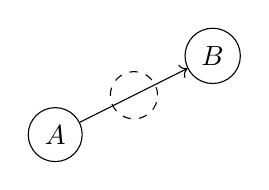
\begin{tikzpicture}
  \node[draw,circle] (a) at (0,0) {$A$};
  \node[draw,circle] (b) at (2,1) {$B$};
  \draw[->] (a) -- (b);
  \draw[dashed] ($(a)!0.5!(b)$) circle (0.3);
\end{tikzpicture}
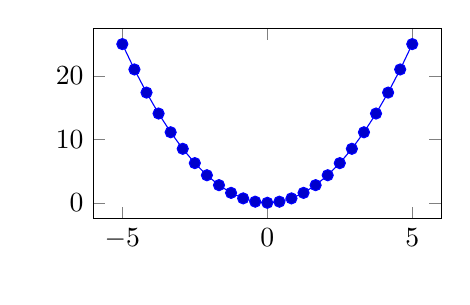
\begin{tikzpicture}
  \begin{axis}[width=6cm,height=4cm]
    \addplot {x^2};
  \end{axis}
\end{tikzpicture}
\end{document}
